% \begin{frame}[t]
%   \frametitle{Dummy}
%   \begin{columns}[T]
%     \begin{column}{0.45\textwidth}
%     \end{column}
%     \begin{column}{0.45\textwidth}
%     \end{column}
%   \end{columns}
% \end{frame}

\begin{frame}[t]
  \frametitle{Symmetric and asymmetric configurations}
  \begin{block}{Two types of polarities}
    MCP readouts are able to work with floating potential.
  \end{block}
  \begin{columns}[T]
    \centering
    \begin{column}{0.45\textwidth}
      \centering
      Symmetric mode:
      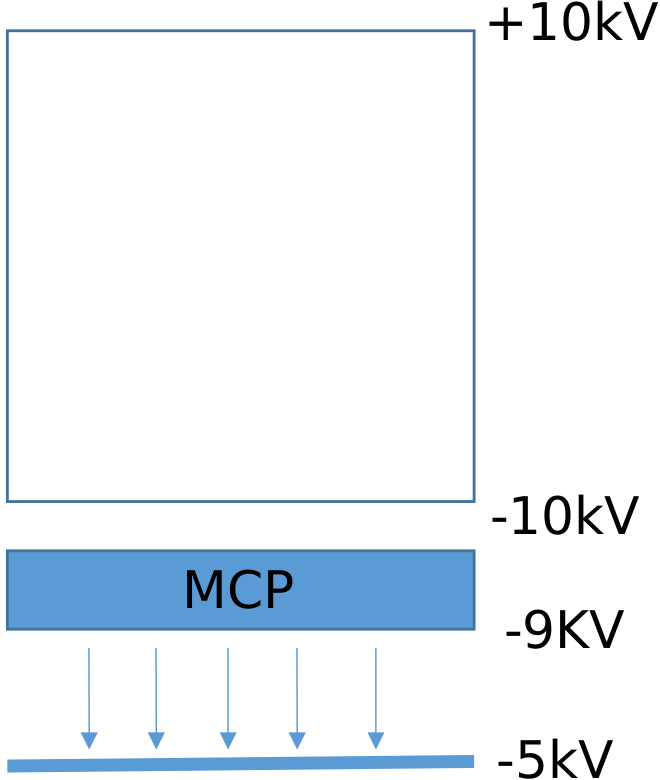
\includegraphics[width=0.7\textwidth]{06_Backup/fig/fig000_SYM}
    \end{column}
    \begin{column}{0.45\textwidth}
      \centering
      Asymmetric mode:
      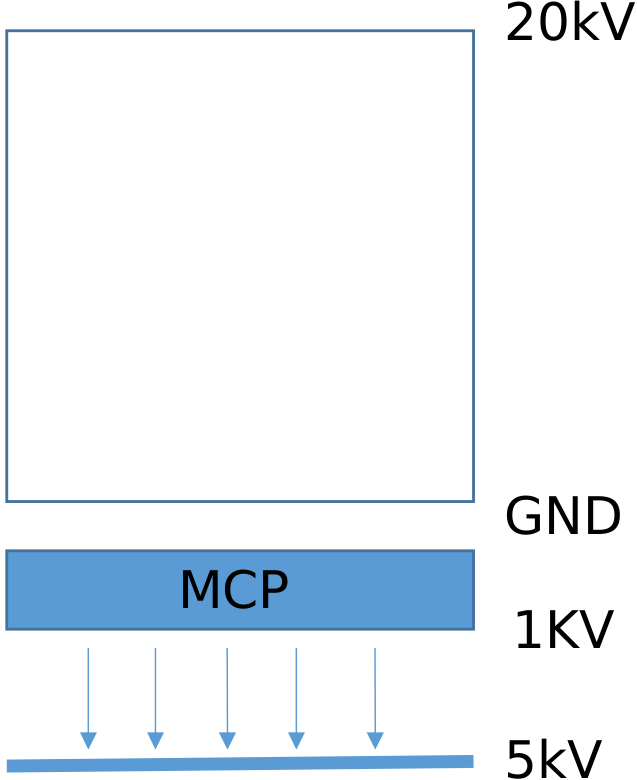
\includegraphics[width=0.7\textwidth]{06_Backup/fig/fig000_ASYM}
    \end{column}
  \end{columns}
\end{frame}

\begin{frame}[t]
  \frametitle{Symmetric and asymmetric configurations}
  \begin{columns}[T]
    \begin{column}{0.45\textwidth}
      \begin{block}{Symmetric mode}
        \begin{itemize}
          \item Good field uniformity without correction
          \item Reduce the maximum voltage for same E field value
          \item Readout protection
        \end{itemize}
      \end{block}
    \end{column}
    \begin{column}{0.45\textwidth}
      \begin{block}{Asymmetric mode}
        \begin{itemize}
          \item Reduce the number of HV channels
          \item Field uniformity is not good without correction
          \item Required higher voltages for same E field value
        \end{itemize}
      \end{block}
    \end{column}
  \end{columns}
  \begin{columns}[T]
    \centering
    \begin{column}{0.45\textwidth}
      \centering
      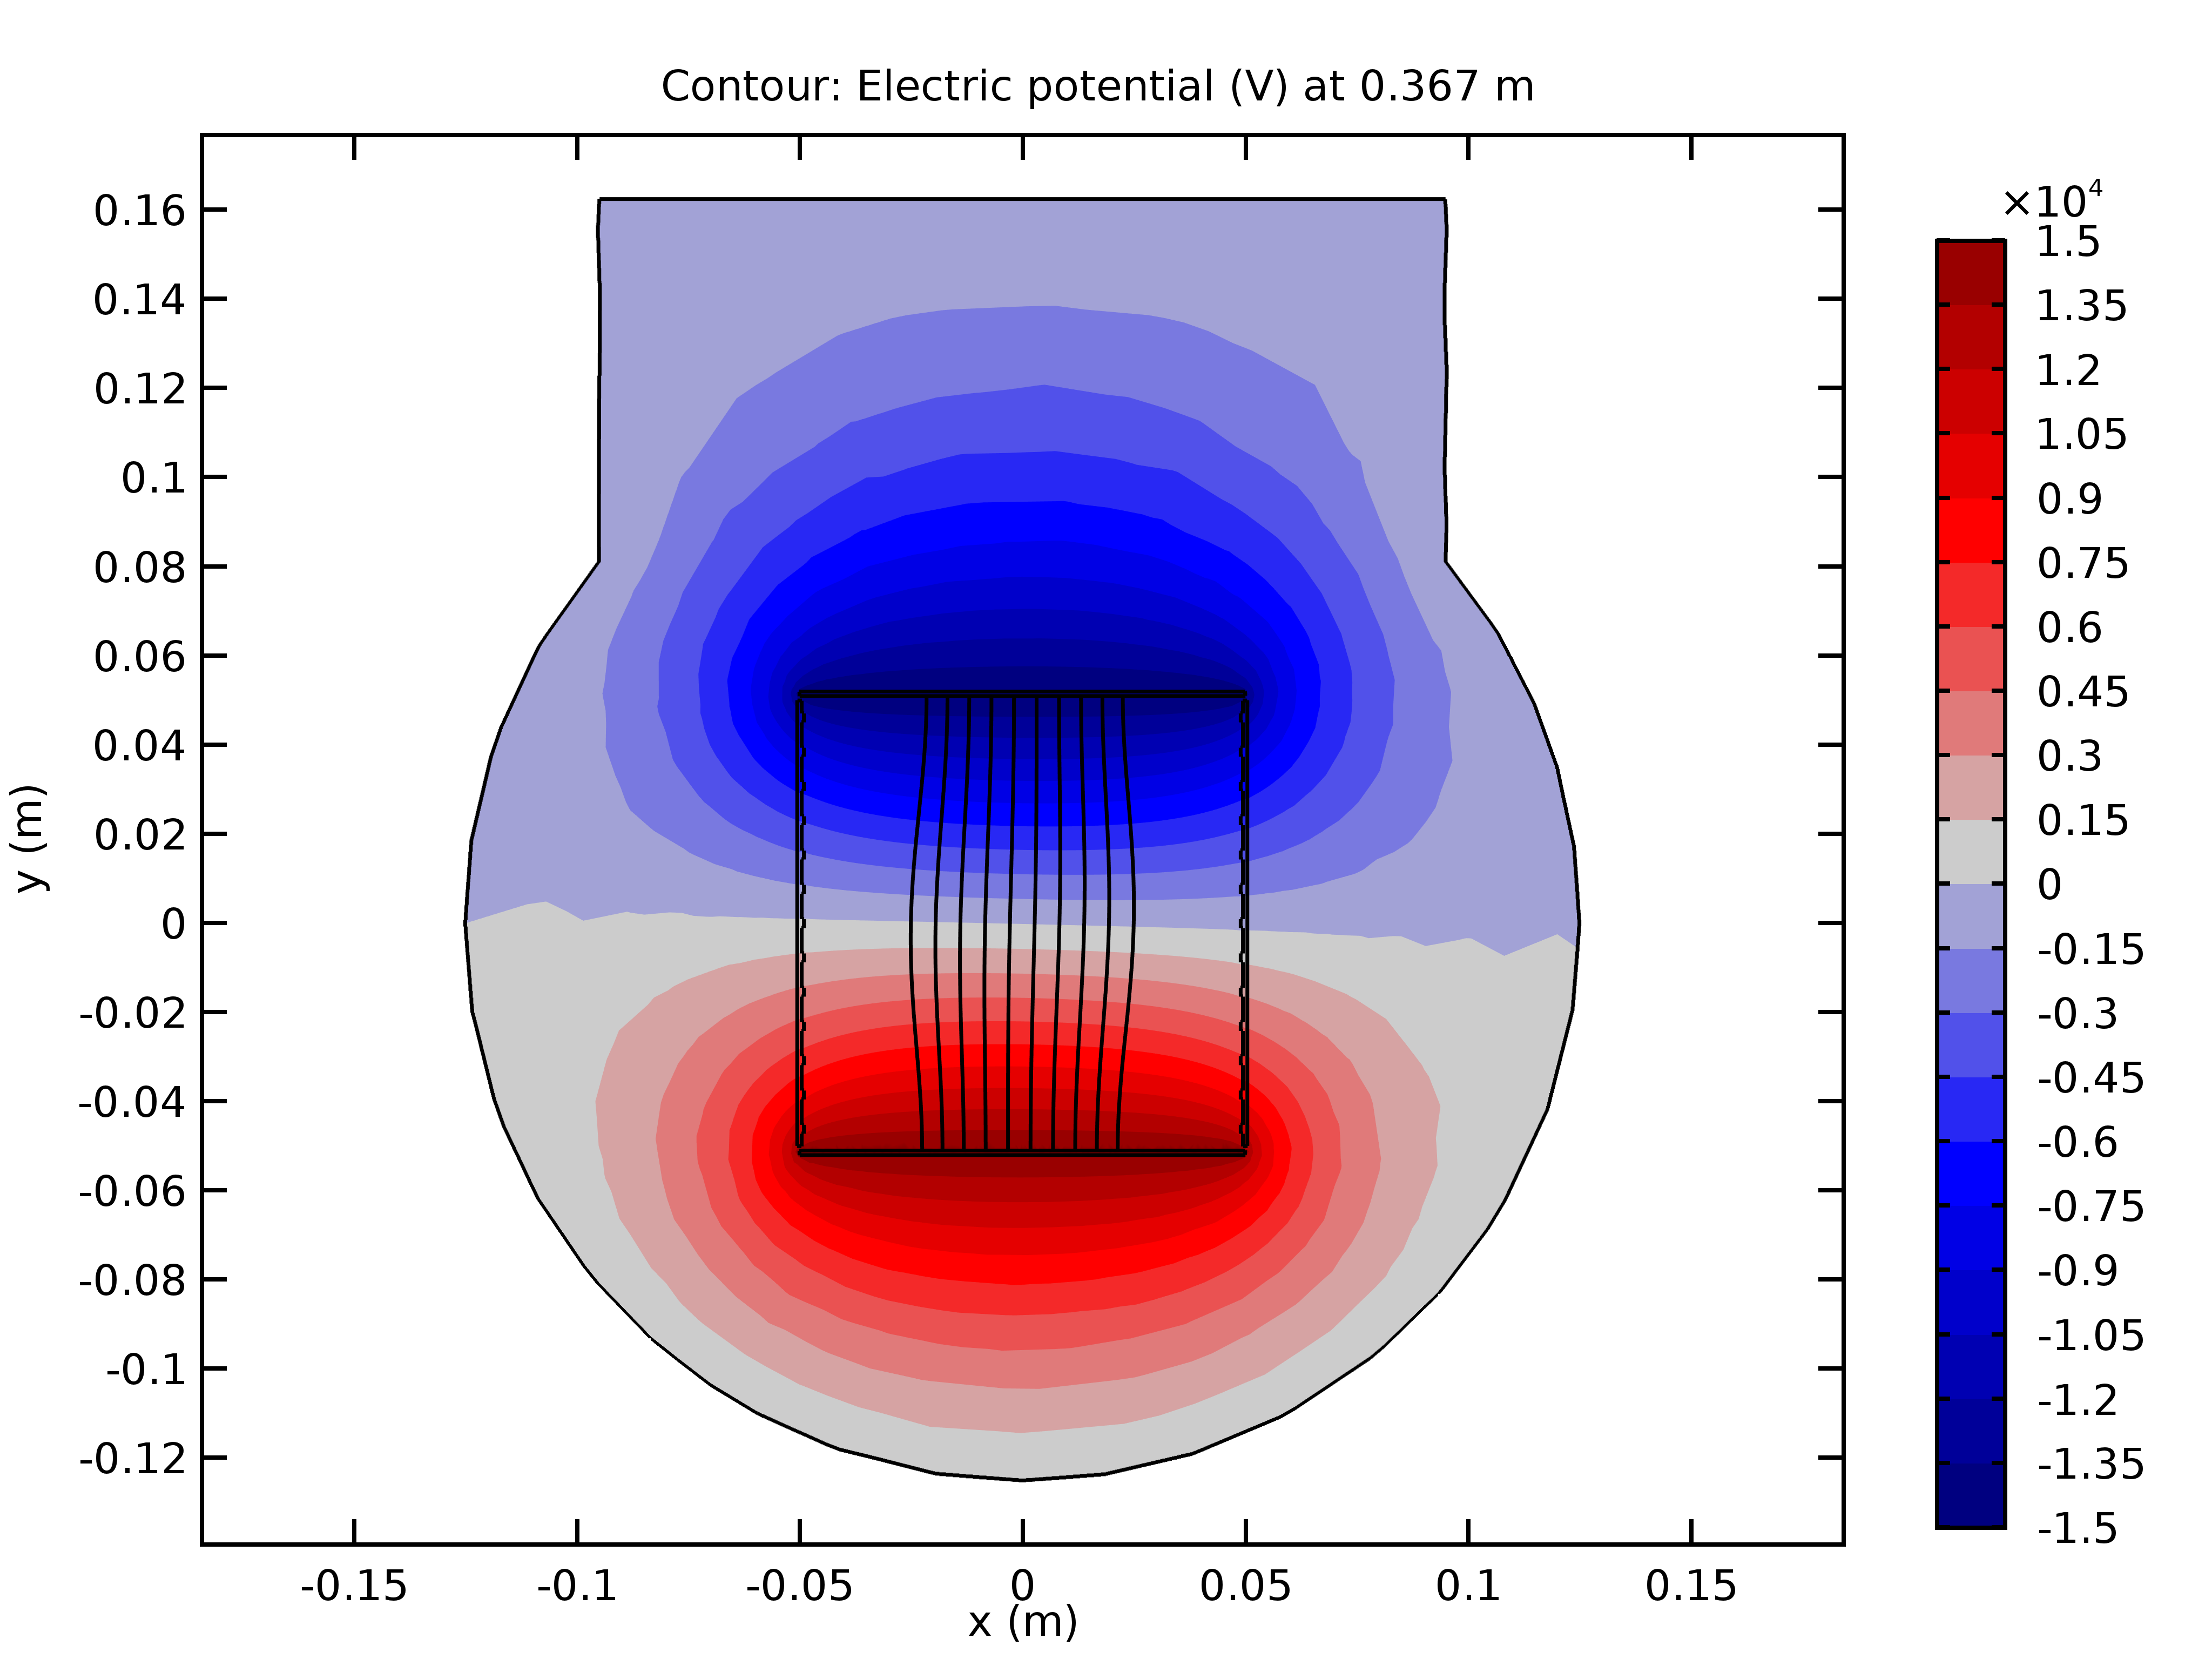
\includegraphics[width=1\textwidth]{06_Backup/fig/fig021_image_asym_sym_b}
    \end{column}
    \begin{column}{0.45\textwidth}
      \centering
      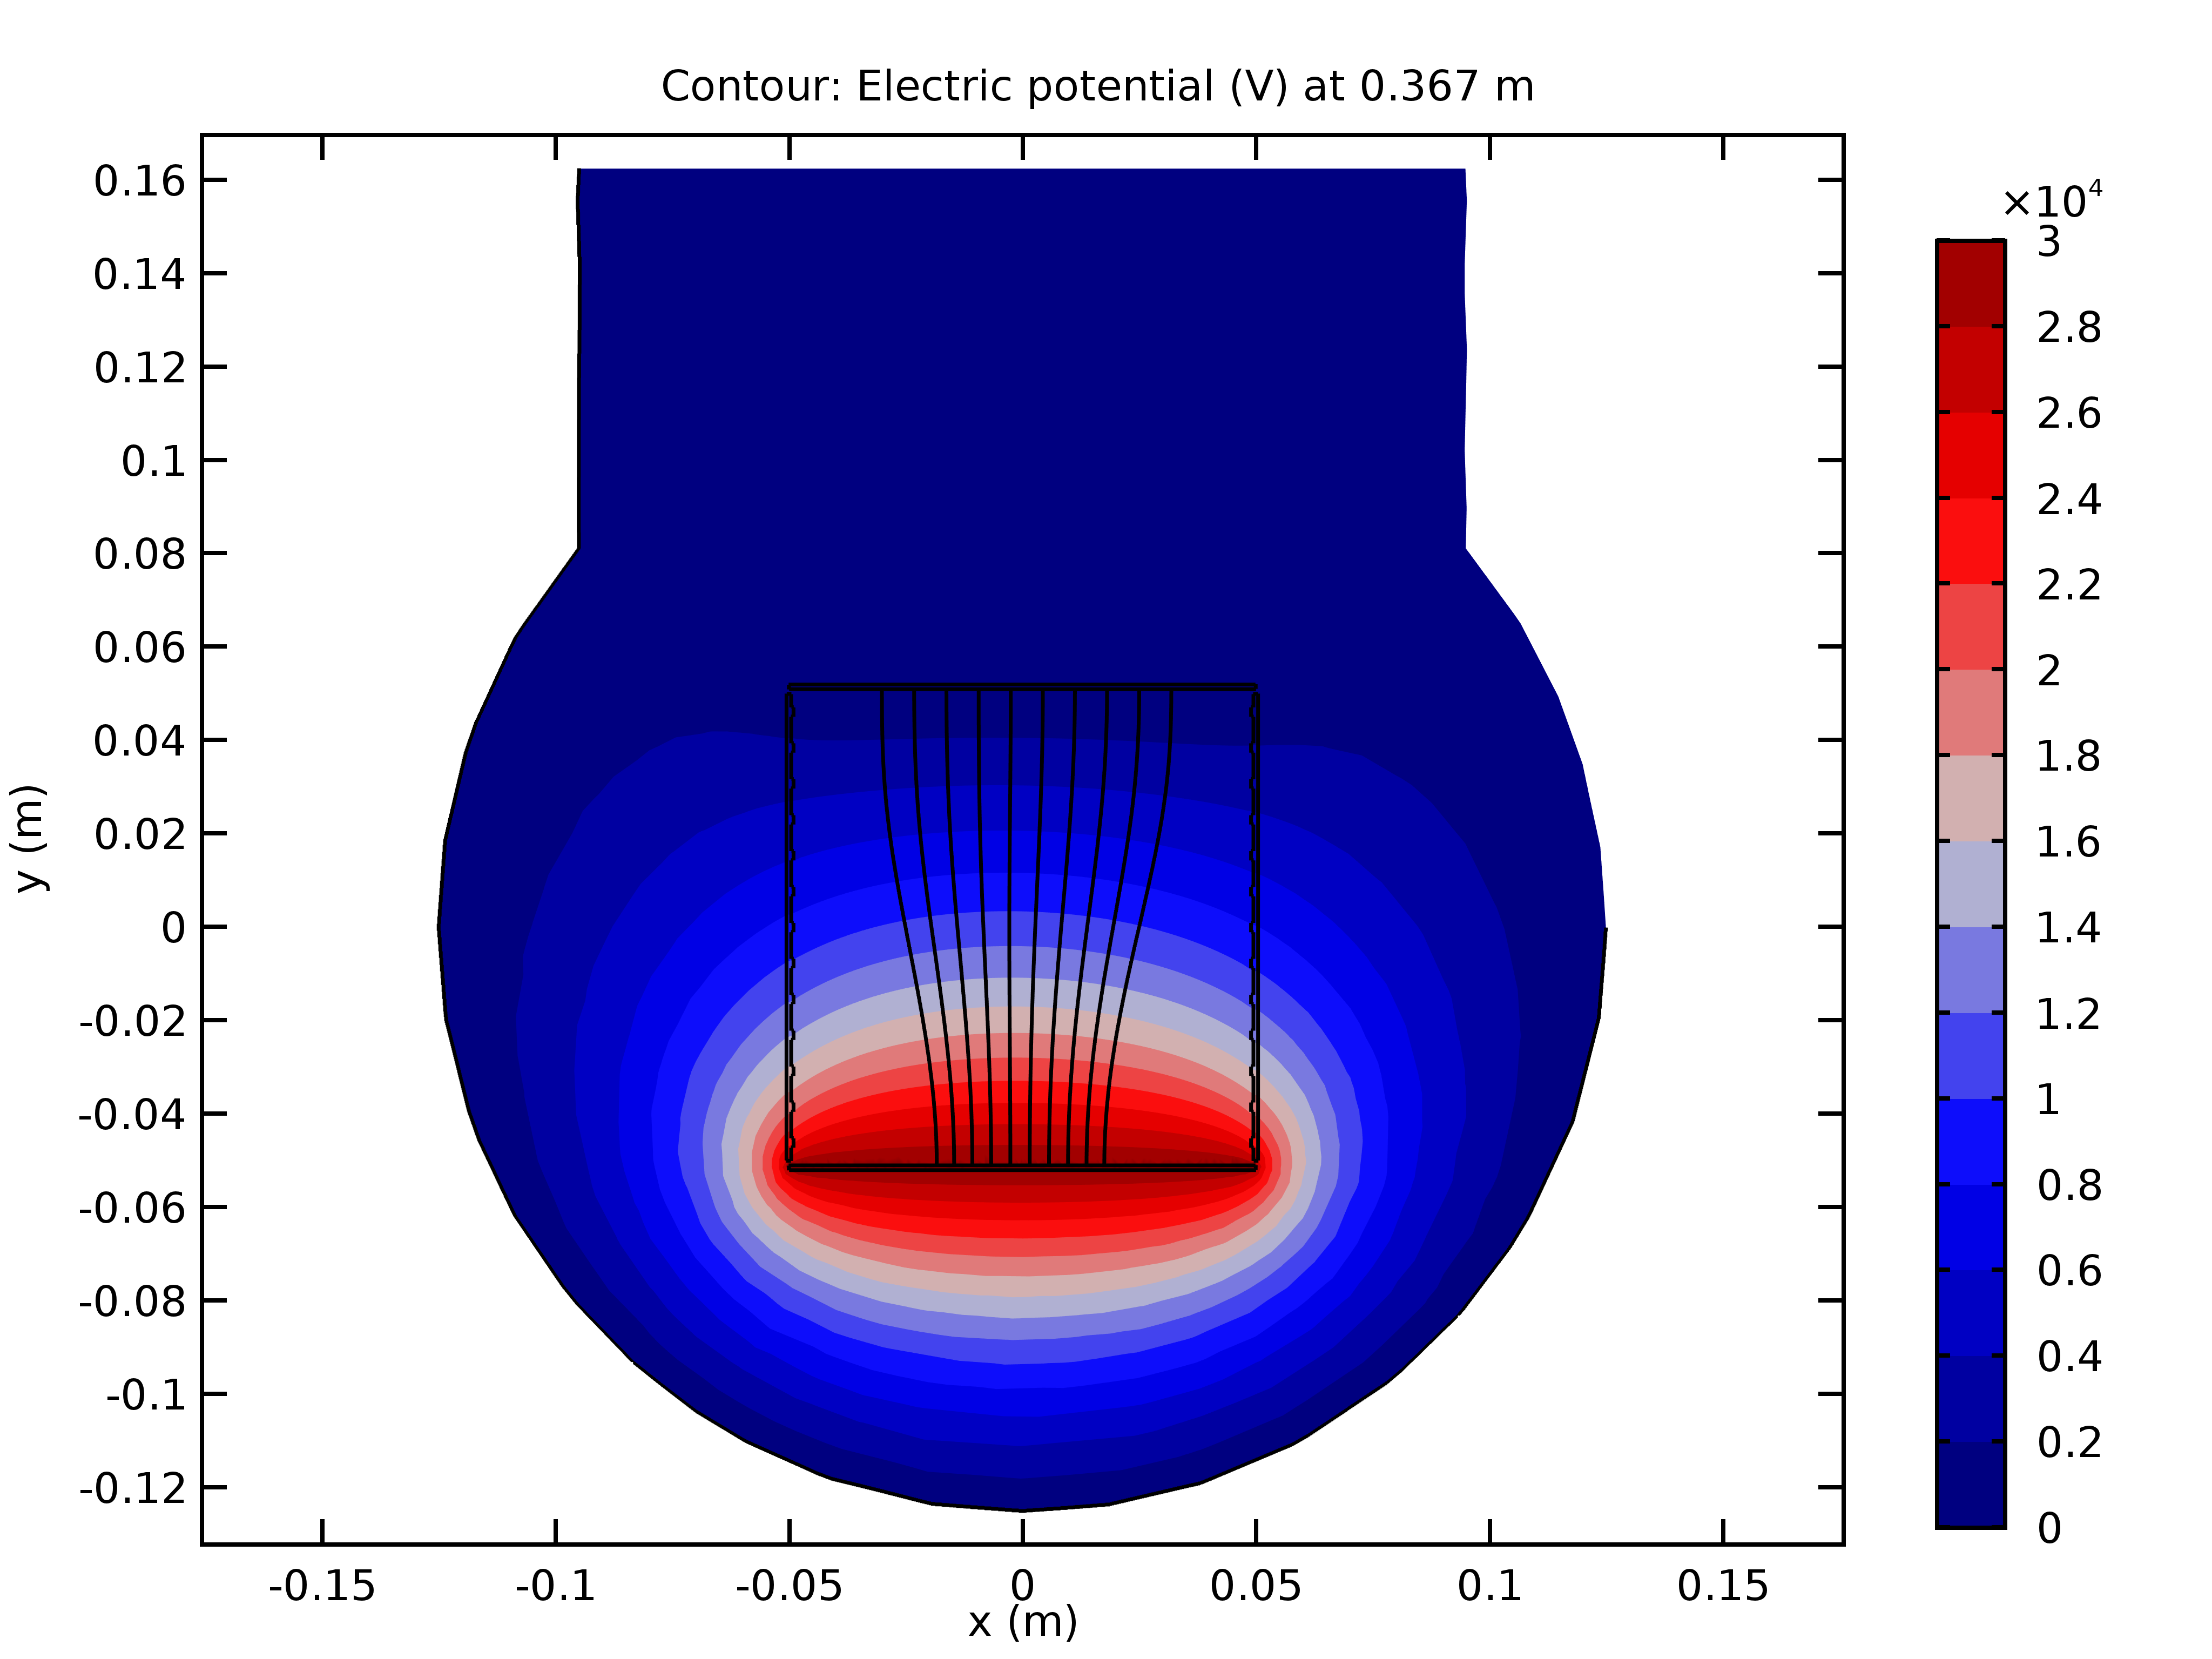
\includegraphics[width=1\textwidth]{06_Backup/fig/fig021_image_asym_sym_a}
    \end{column}
  \end{columns}
\end{frame}

\begin{frame}[t]
  \frametitle{COMSOL simulation checks}
  \begin{block}{Data Processing}
    However a symmetric IPM can be switched to an asymmetric IPM $\implies$ the field is intentionally degraded.
  \end{block}

  \begin{block}{This can be simulated by COMSOL}
    \begin{enumerate}
      \item Compute field of a symmetric IPM powered with symmetric high voltages.
      \item Compute field of a symmetric IPM powered with asymmetric high voltages.
      \item Compute the ratio in size and position of the two models.
    \end{enumerate}
  \end{block}

  \begin{block}{Check process}
    \begin{enumerate}
      \item Symmetric IPM powered with symmetric high voltages.
      \item Several position and size are recorded for different steerer values.
      \item Symmetric IPM powered with asymmetric high voltages.
      \item Record position and size with same steerer values.
      \item Compute the ratio in size and position between the two measurements.
    \end{enumerate}
  \end{block}
\end{frame}

\begin{frame}[t]
  \frametitle{COMSOL simulation checks}
  \begin{block}{From simulations, the following are observed:}
    \begin{itemize}
      \item The profile is thinner in asymmetric.
      \item In the asymmetric mode the field pulls the particle in the center of IPM.
    \end{itemize}
  \end{block}
  \begin{columns}[T]
    \begin{column}{0.45\textwidth}
      Ratio size:
      \centering
      \only<1>{%
        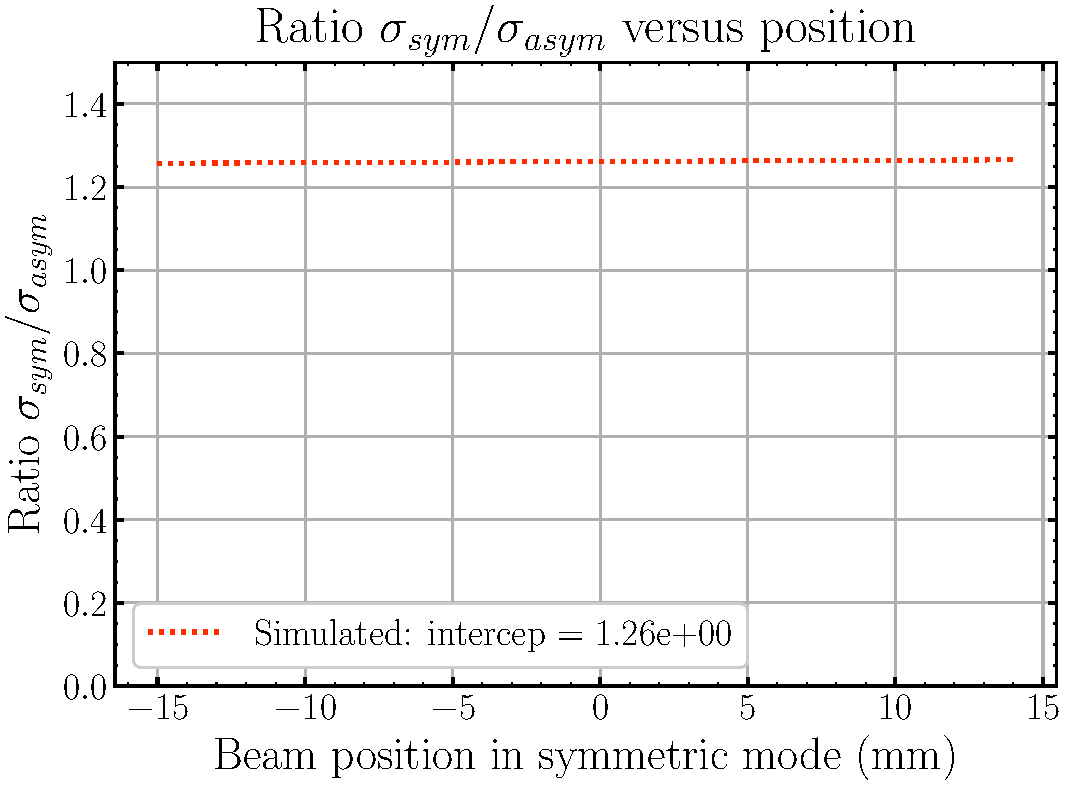
\includegraphics[width=1\textwidth]{06_Backup/fig/fig000_fieldcomp_b1}%
      }%
      \only<2>{%
        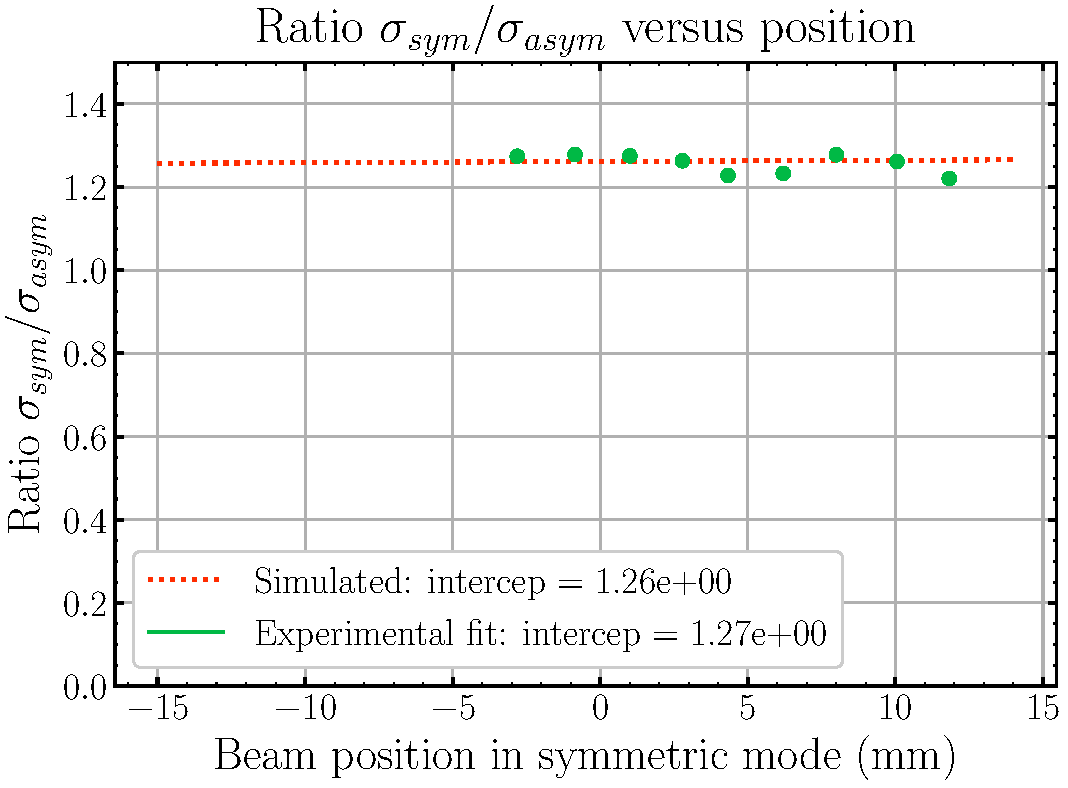
\includegraphics[width=1\textwidth]{06_Backup/fig/fig000_fieldcomp_b2}%
      }%
    \end{column}
    \begin{column}{0.45\textwidth}
      Ratio position:
      \centering
      \only<1>{%
        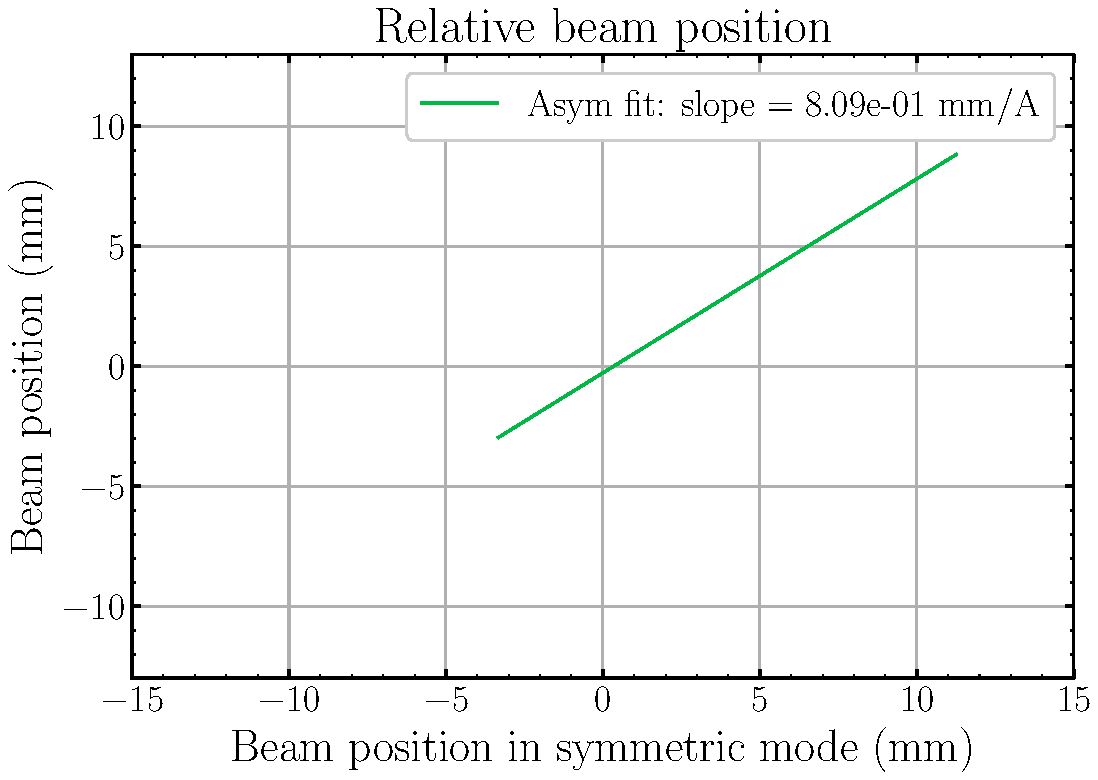
\includegraphics[width=1\textwidth]{06_Backup/fig/fig000_fieldcomp_a1}%
      }%
      \only<2>{%
        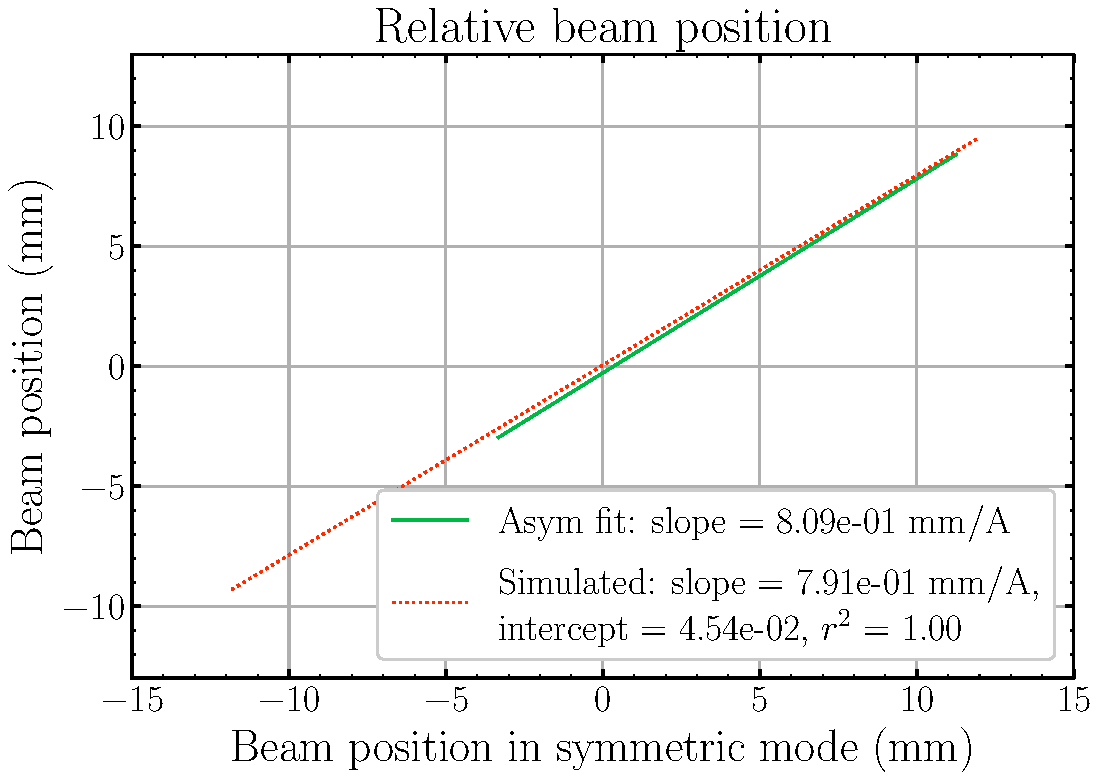
\includegraphics[width=1\textwidth]{06_Backup/fig/fig000_fieldcomp_a2}%
      }%
    \end{column}
  \end{columns}
\end{frame}

% \begin{frame}[t]
%   \frametitle{More information Geant4 simulation}
%   \begin{columns}[T]
%     \begin{column}{0.45\textwidth}
%       \begin{block}{Silicon simulation}
%         \begin{itemize}
%           \item 10000 particles
%           \item Cube sliced into several layer
%           \item Physic list: emlivermore
%         \end{itemize}
%       \end{block}
%     \end{column}
%     \begin{column}{0.45\textwidth}
%       \begin{block}{ESS simulation}
%         CAD import:
%         \begin{enumerate}
%           \item STEP verification with FreeCAD.
%           \item STEP to STL via script using FreeCAD python lib.
%           \item (optional) Reduce STL vertices.
%           \item Geant4 import with CADMesh lib.
%         \end{enumerate}
%         \begin{itemize}
%           \item
%         \end{itemize}
%       \end{block}
%     \end{column}
%   \end{columns}
% \end{frame}

% \begin{frame}[t]
%   \frametitle{Convergence during a run}

% \end{frame}

% \begin{frame}[t]
%   \frametitle{Space charge at IPHI}
%   \begin{block}{Space charge effect also occurs at IPHI}
%     But different beam conditions:
%     \begin{itemize}
%       \item $\sigma_x, \sigma_y$
%       \item $\sigma_z$
%     \end{itemize}
%   \end{block}
%   \begin{block}{Conclusion}

%   \end{block}
% \end{frame}

\begin{frame}[t]
  \frametitle{Space charge at IPHI}
  \begin{block}{Simulation checks}
    The space charge code has been checked at IPHI by changing extraction field at $i_{beam}=30\,\mathrm{mA}$. The $\sigma_{y}$ was measured whereas  $\sigma_{z}=29\,\mathrm{mm}$ and $\sigma_{x}=4\,\mathrm{mm}$ were estimated via TraceWin.
  \end{block}
  \begin{center}
    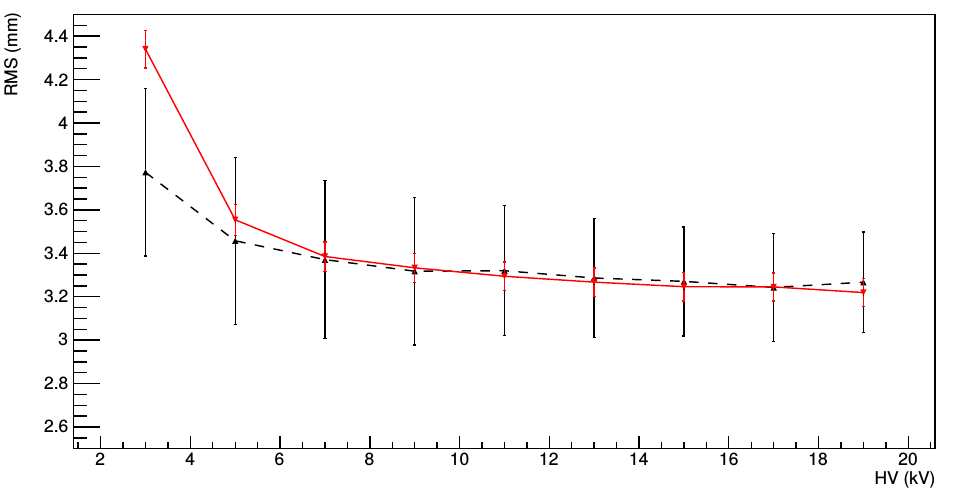
\includegraphics[width=0.8\textwidth]{06_Backup/fig/fig000_SC_IPHI_check}
  \end{center}
  \begin{textblock*}{4cm}(8cm,4.5cm)      
    Experimental $\sigma_{y}$
    
    \textcolor{red}{Simulated $\sigma_{y}$}
  \end{textblock*}
\end{frame}

\begin{frame}[t]
  \frametitle{More on campaigns}
  \begin{block}{Two campaigns}
    Two campaigns with different IPM configuration. Some spark issues during the first campaign. The design has been improved for a second campaign.
  \end{block}
  \begin{tabularx}{\linewidth}{XXX}
    \toprule
                  & First campaign      & Second campaign     \\
    \midrule
    Starting date & 19/02/2018          & 14/09/2018          \\
    First profile & 01/03/2018          & 14/09/2018          \\
    Ending date   & 13/04/2018          & 26/10/2018          \\
    IPM 1         & Linear strips (Y)   & Gaussian strips (X) \\
    IPM 2         & Hamamatsu MCP (Y)   & Photonis MCP (Y)    \\
    IPM 3         & Gaussian strips (Y) & Linear strips (Y)   \\
    \bottomrule
  \end{tabularx}
  \begin{columns}[T]
    \begin{column}{0.45\textwidth}
    \end{column}
    \begin{column}{0.45\textwidth}
    \end{column}
  \end{columns}
\end{frame}

\begin{frame}[t]
  \frametitle{IPM at low energies}
  \begin{block}{Limits of non invasive}
    At $3\,\mathrm{MeV}$ the extraction field of the IPM can deviate the beam.
    The shift induced by IPM1 can be measured with the IPM1 and IPM2. The variation is not observed by the BPM.
  \end{block}
  \begin{columns}[T]
    \begin{column}{0.45\textwidth}
      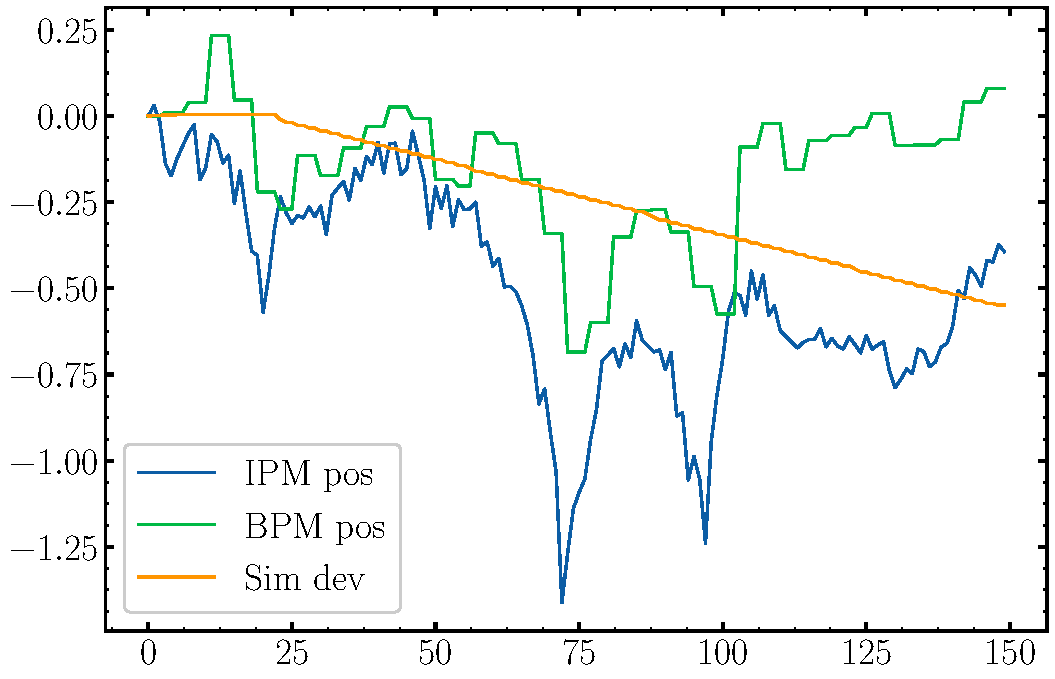
\includegraphics[width=1\textwidth]{06_Backup/fig/fig000_dev_IPM_BPM}
    \end{column}
    \begin{column}{0.45\textwidth}
      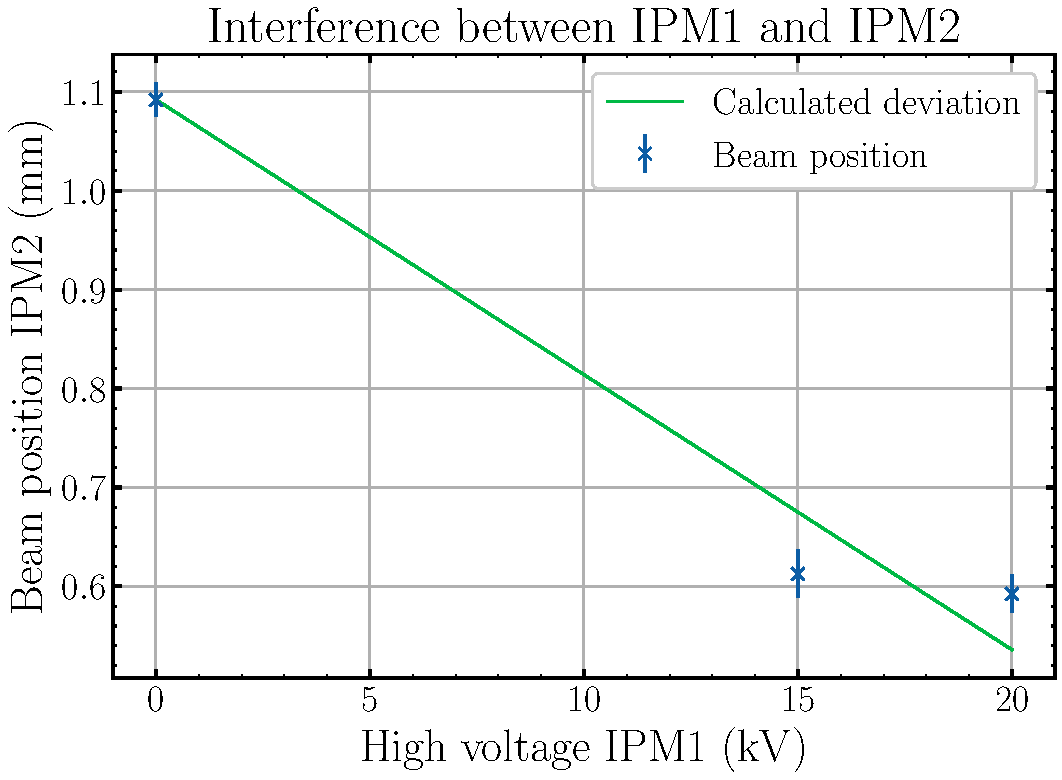
\includegraphics[width=1\textwidth]{06_Backup/fig/fig000_cross_position}
    \end{column}
  \end{columns}
\end{frame}

\begin{frame}[t]
  \frametitle{Phosphorus screen}
  \begin{columns}[T]
    \begin{column}{0.45\textwidth}
      \begin{block}{Phosphorus screens}
        Two screens have been tested:
        \begin{itemize}
          \item P43: slow, efficient ($100\,\%$)
          \item P46: fast, efficient ($30\,\%$)
        \end{itemize}
      \end{block}
      \only<1>{P43 gain:%

      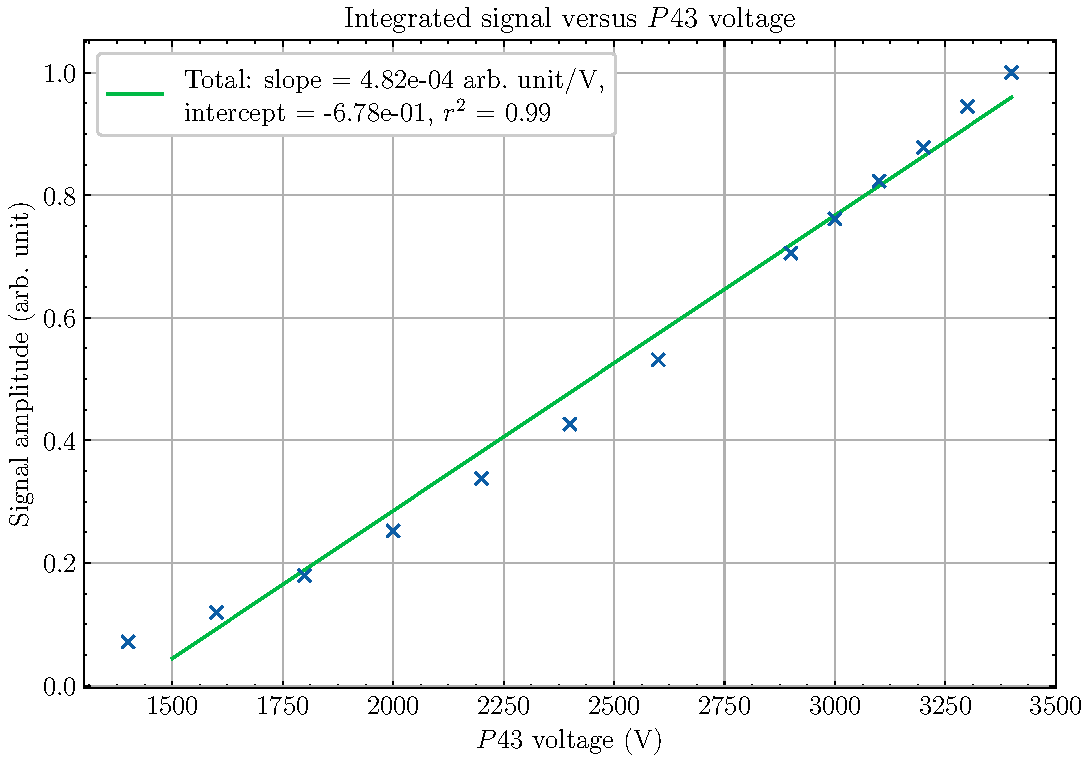
\includegraphics[width=1\textwidth]{06_Backup/fig/fig000_P43_gain}%
      }%
      \only<2>{P43 influence size:%

      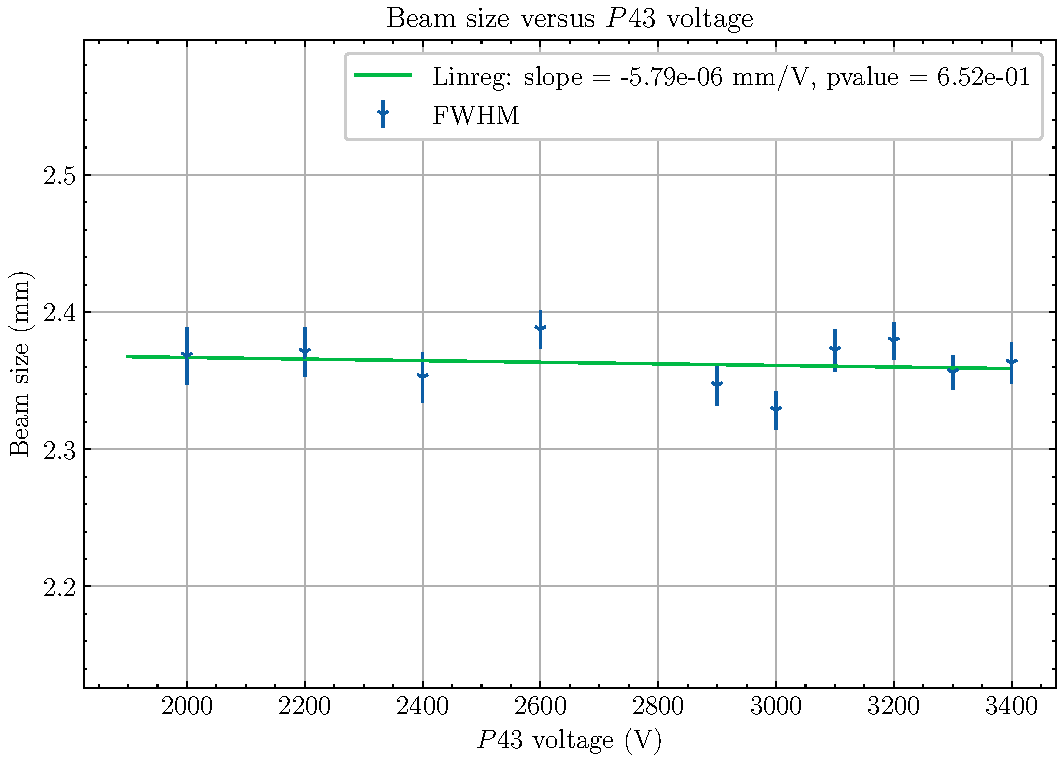
\includegraphics[width=1\textwidth]{06_Backup/fig/fig000_P43_size}%
      }%
      \only<3>{P46 gain:%

      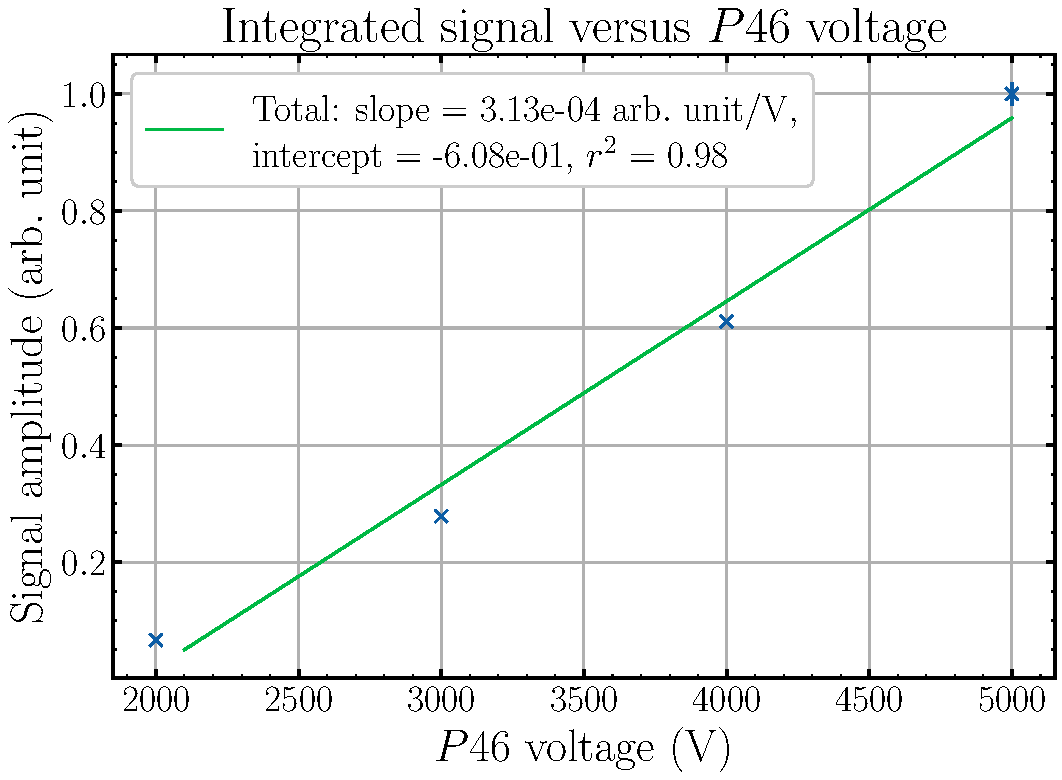
\includegraphics[width=1\textwidth]{06_Backup/fig/fig000_P46_gain}%
      }%
      \only<4>{P46 influence size:%

      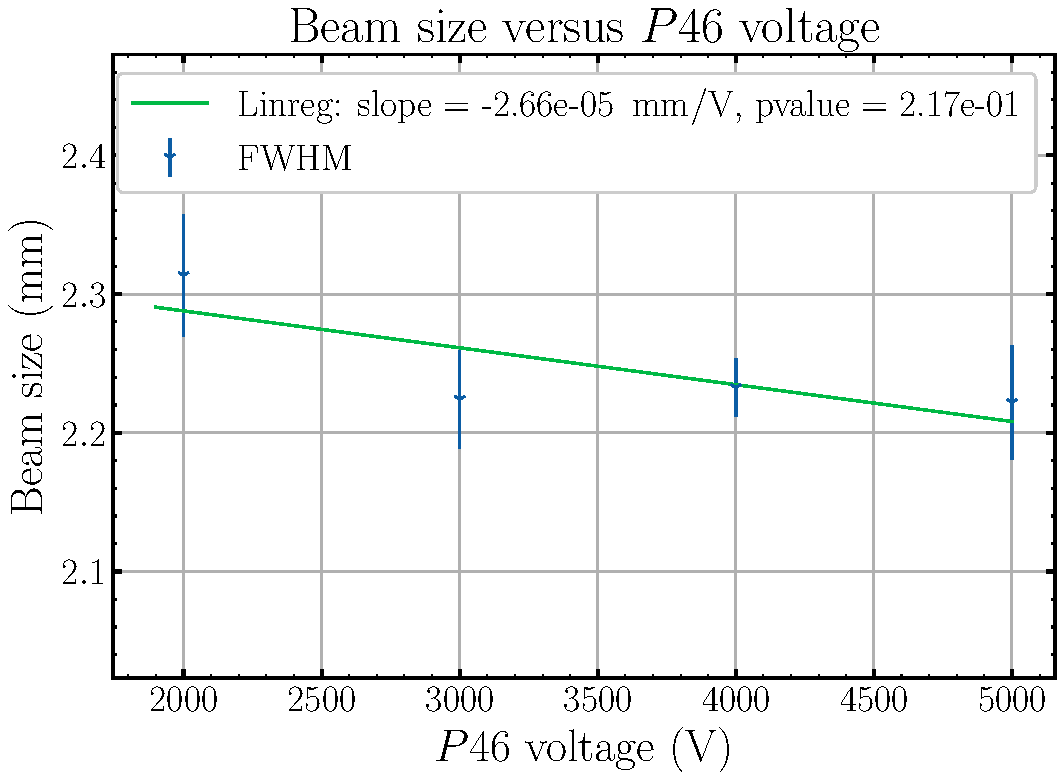
\includegraphics[width=1\textwidth]{06_Backup/fig/fig000_P46_size}%
      }%
    \end{column}
    \begin{column}{0.45\textwidth}
      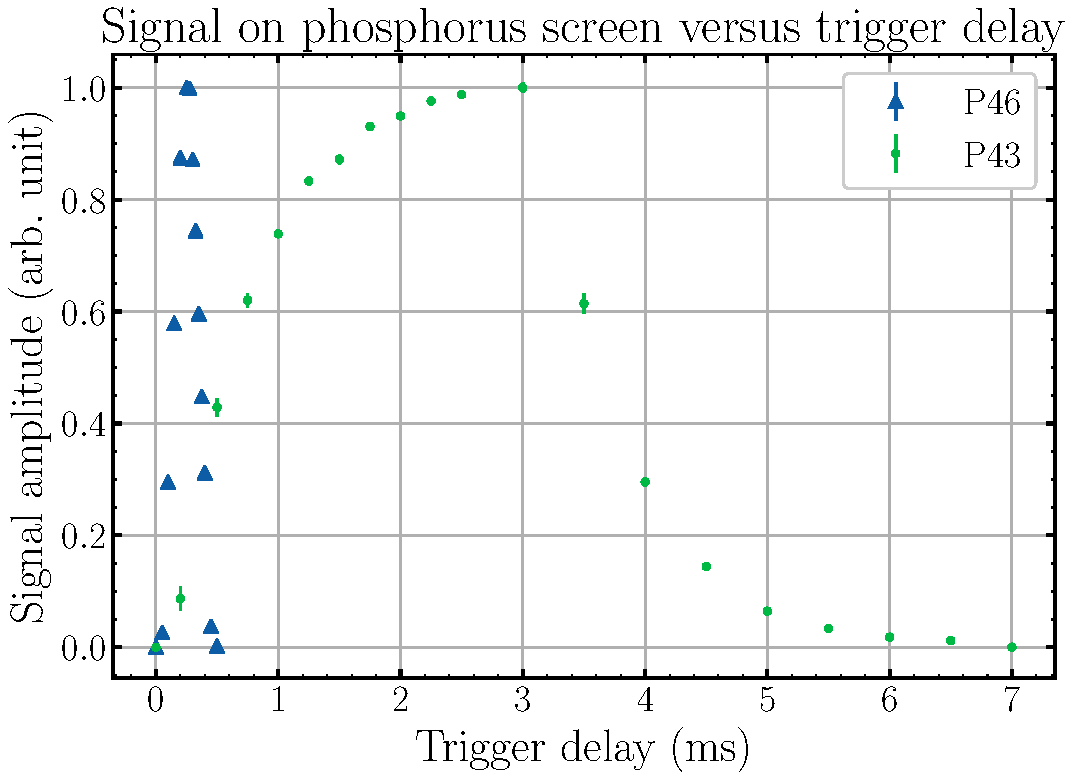
\includegraphics[width=1\textwidth]{06_Backup/fig/fig000_timing}
      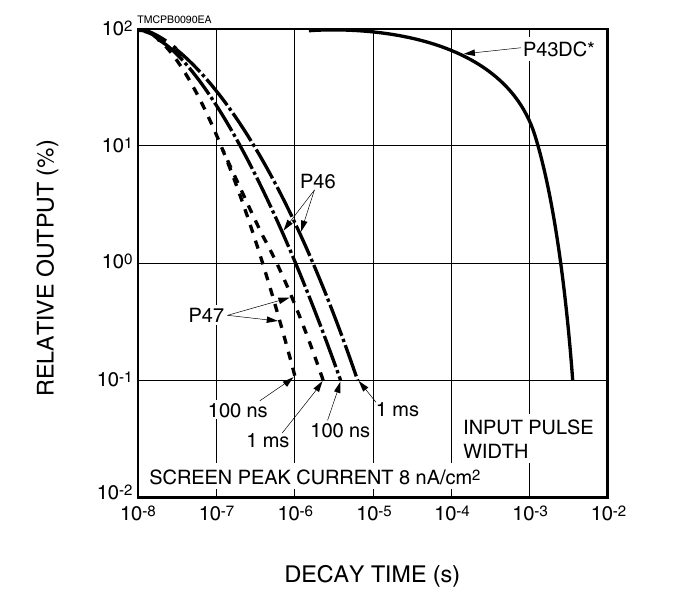
\includegraphics[width=1\textwidth]{06_Backup/fig/fig000_Hamamatu_phos}
    \end{column}
  \end{columns}
\end{frame}

\begin{frame}[t]
  \frametitle{Screens}
  \begin{block}{Interceptive screens}
    A scintillator screen is inserted directly on the beam path.
    The profile on screen is recorded by a camera.
  \end{block}
  \begin{tabularx}{\linewidth}{XXXX}
    \toprule
    Property                            & $\mathrm{Prelude}420$ & $YAG:Ce$ & $BGO$  \\
    %                                    & $Lu^{1.8}Y.^{2}SiO^{5}:Ce$ & $Y_{3}Al_{5}O_{12}(Ce)$ & $Bi_{4}Ge_{3}O_{12}$ \\
    \midrule
    $\rho$ ($\mathrm{g/cm^3}$)          & $7.1$                 & $4.57$   & $7.13$ \\
    Light yield ($\mathrm{\gamma/keV}$) & $33$                  & $8$      & $8-10$ \\
    $\lambda$ ($\mathrm{nm}$)           & $420$                 & $550$    & $480$  \\
    $t_{decay}$ ($\mathrm{ns}$)         & $36$                  & $70$     & $300$  \\
    \bottomrule
  \end{tabularx}
  \centering
  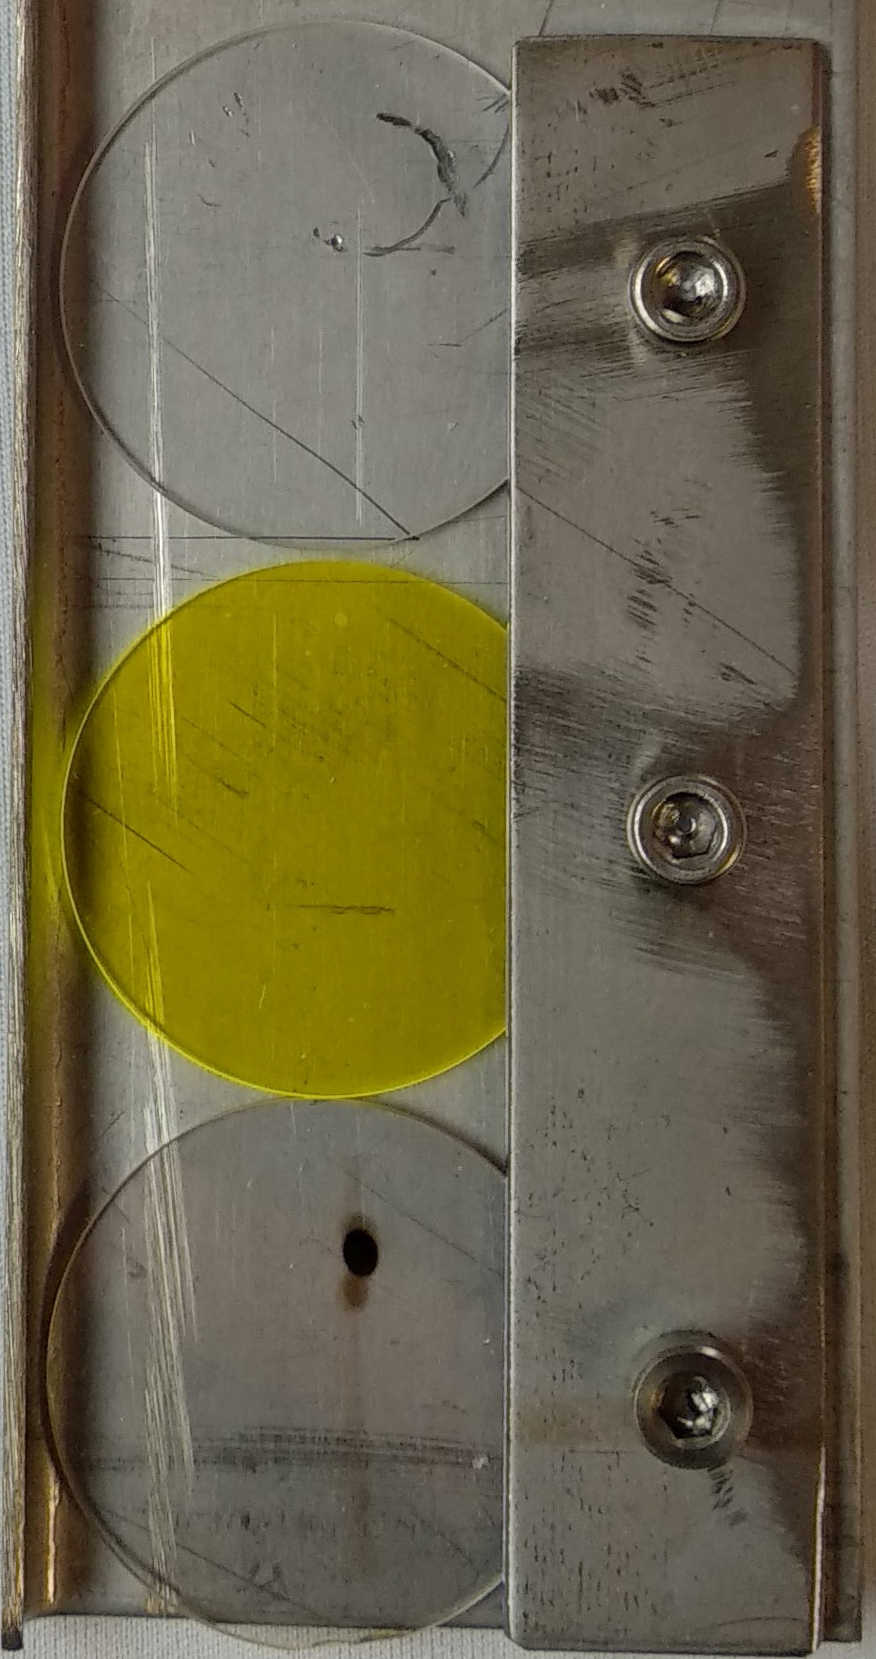
\includegraphics[angle=90,width=0.5\textwidth]{06_Backup/fig/fig000_ecran}
\end{frame}

\begin{frame}[t]
  \frametitle{Screens}
  \begin{block}{IPHI is powerfull even at low duty cycle}
    Two screens died in few pulses for $i_{beam} < 5 \, \mathrm{mA}$ and $t_{pulse} < 200 \, \mathrm{\mu s}$
  \end{block}
  \begin{columns}[T]
    \begin{column}{0.45\textwidth}
      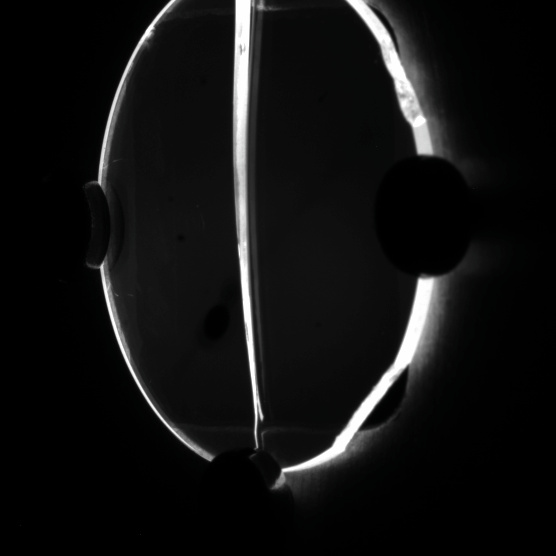
\includegraphics[width=1\textwidth]{06_Backup/fig/fig000_rip_a}
    \end{column}
    \begin{column}{0.45\textwidth}
      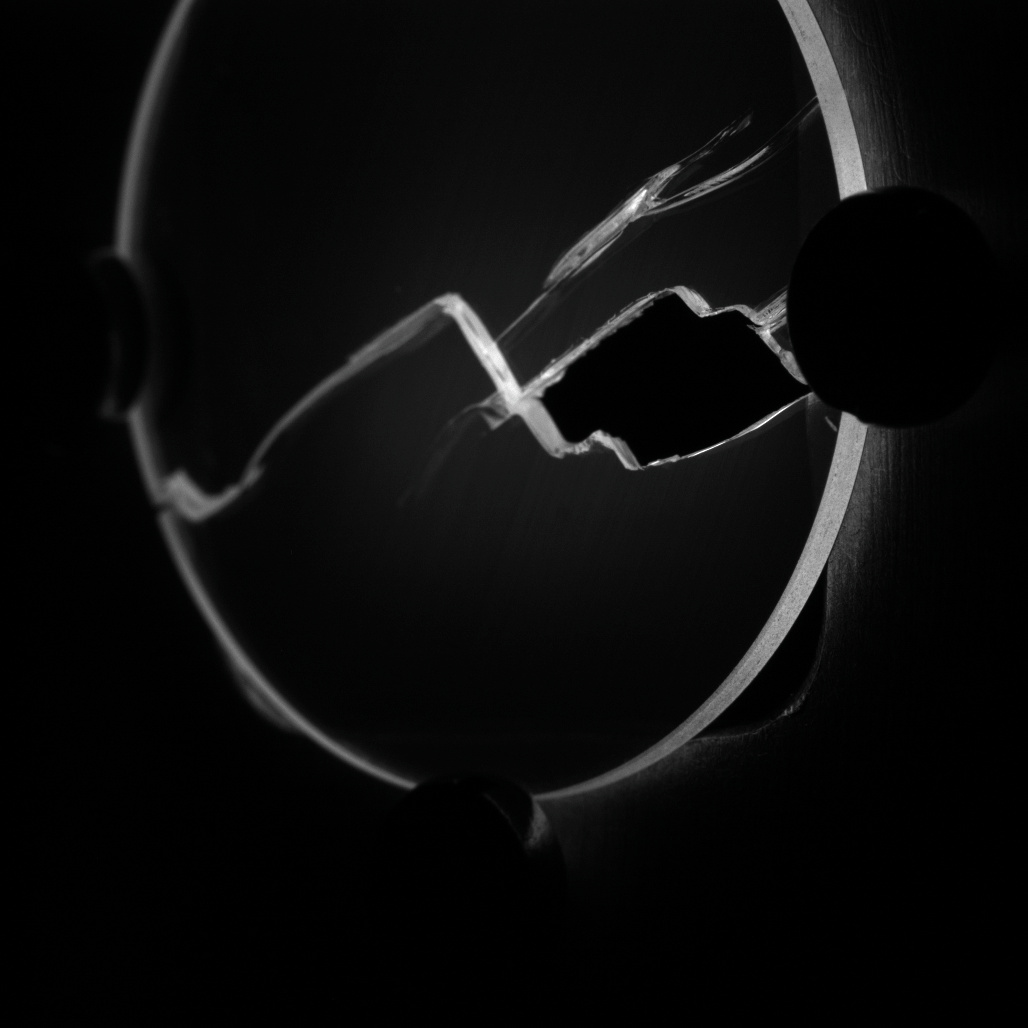
\includegraphics[width=1\textwidth]{06_Backup/fig/fig000_rip_b}
    \end{column}
  \end{columns}
\end{frame}

\begin{frame}[t]
  \frametitle{$Y_{3}Al_{5}O_{12}(Ce)$: The survivor}
  \begin{block}{The screen observed the profile during the two campaign}
     \begin{itemize}
       \item First campaign: the dipole dispersion is visible.
       \item Second campaign: the dipole dispersion is not visible $\rightarrow$ cut by a collimator.
     \end{itemize}
  \end{block}
  \begin{columns}[T]
    \begin{column}{0.45\textwidth}
      \only<1>{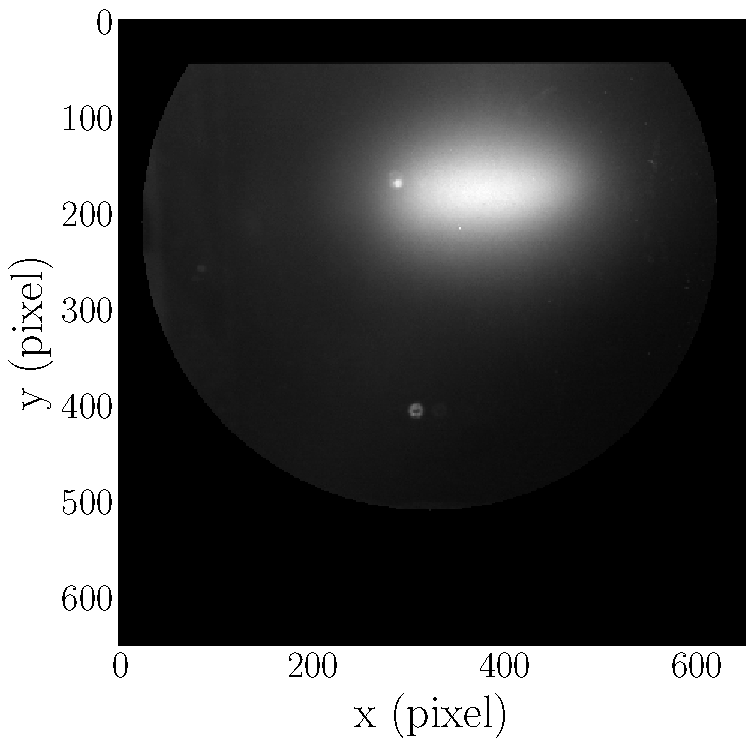
\includegraphics[width=1\textwidth]{06_Backup/fig/fig000_ScreenBeam_a}}
      \only<2>{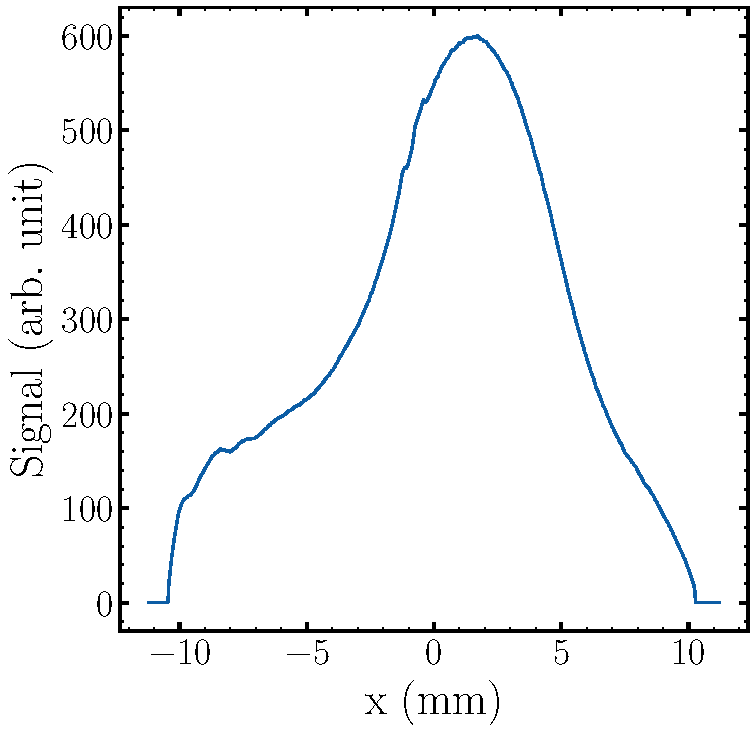
\includegraphics[width=1\textwidth]{06_Backup/fig/fig000_ScreenBeam_b}}
      \only<3>{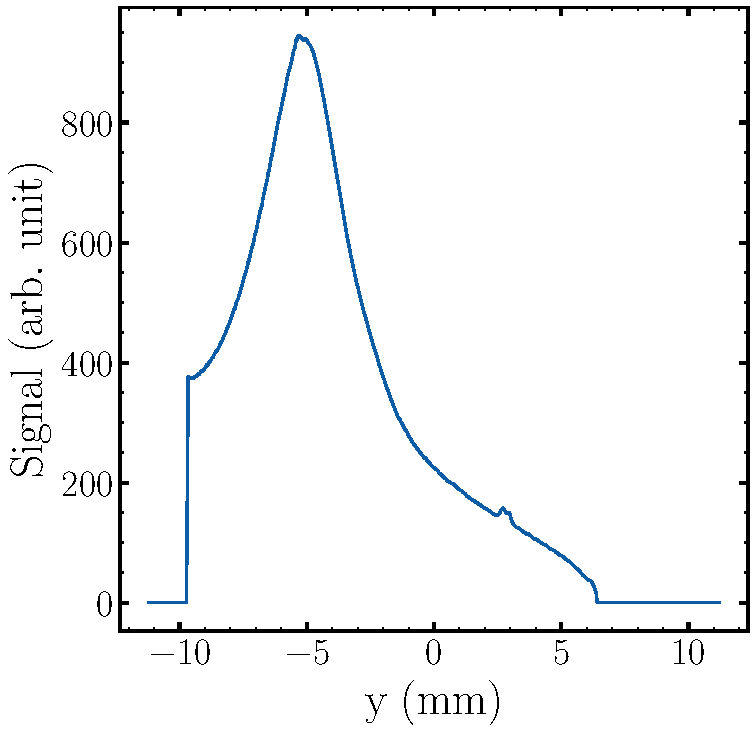
\includegraphics[width=1\textwidth]{06_Backup/fig/fig000_ScreenBeam_c}}
    \end{column}
    \begin{column}{0.45\textwidth}
      \only<1>{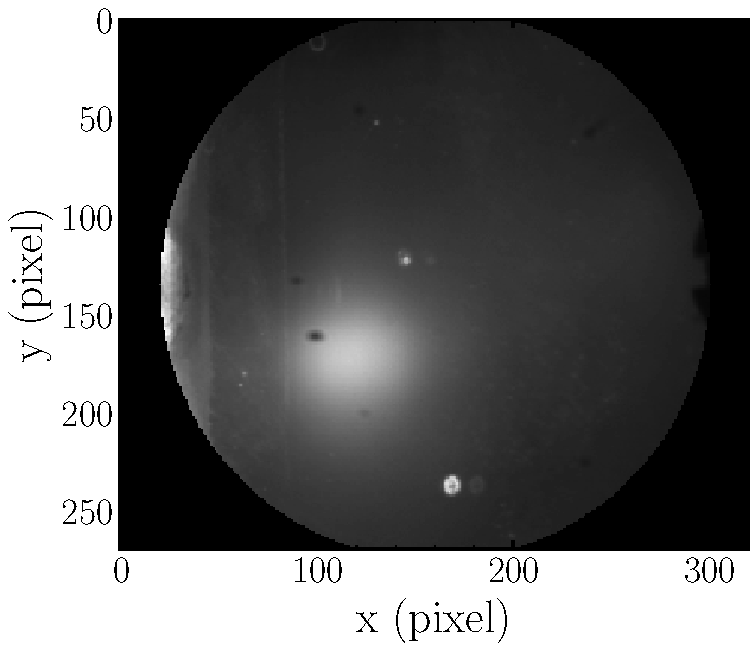
\includegraphics[width=1\textwidth]{06_Backup/fig/fig000_ScreenBeam2_a}}
      \only<2>{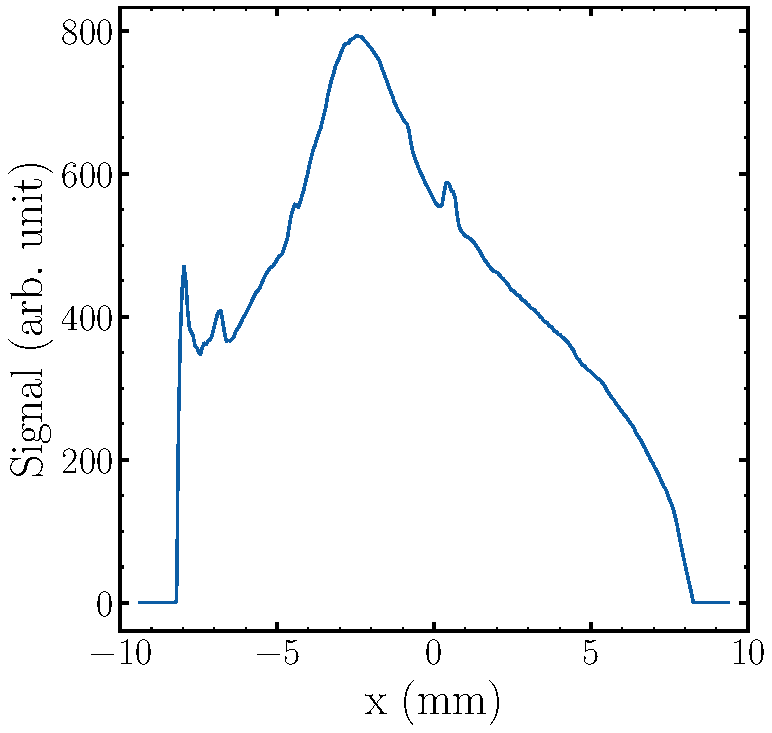
\includegraphics[width=1\textwidth]{06_Backup/fig/fig000_ScreenBeam2_b}}
      \only<3>{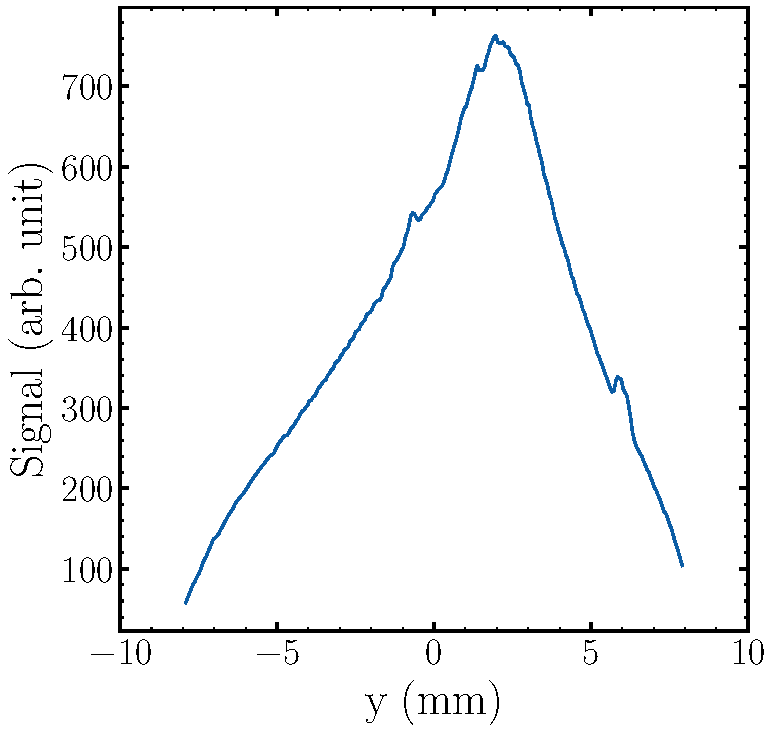
\includegraphics[width=1\textwidth]{06_Backup/fig/fig000_ScreenBeam2_c}}
    \end{column}
  \end{columns}
\end{frame}

\begin{frame}[t]
  \frametitle{FPM}
  \begin{block}{Background light}
    Too many parasitic light inside vessel.

    Even with a black coated sleeve.
  \end{block}
  \begin{columns}[T]
    \begin{column}{0.45\textwidth}
      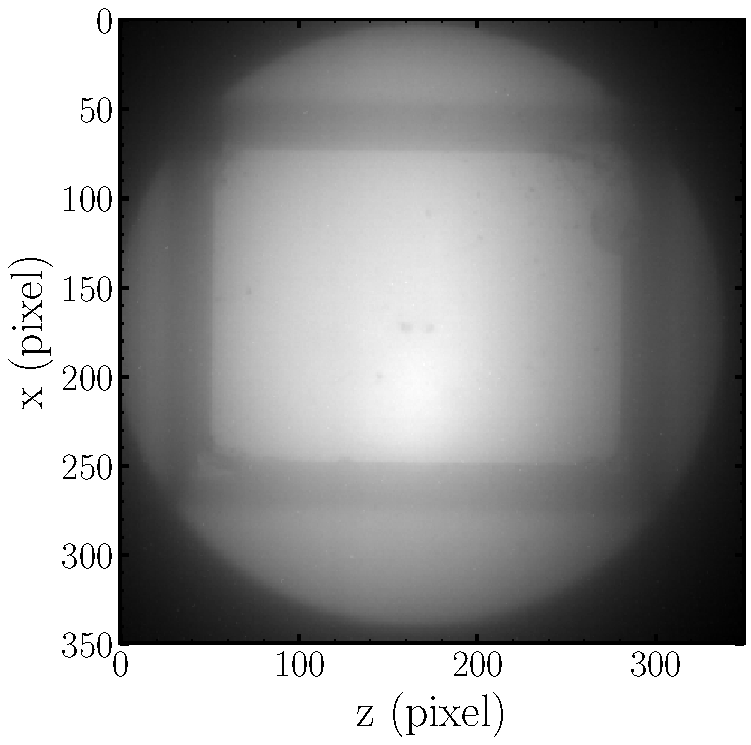
\includegraphics[width=\textwidth]{06_Backup/fig/fig000_FPM_a.pdf}
    \end{column}
    \begin{column}{0.45\textwidth}
      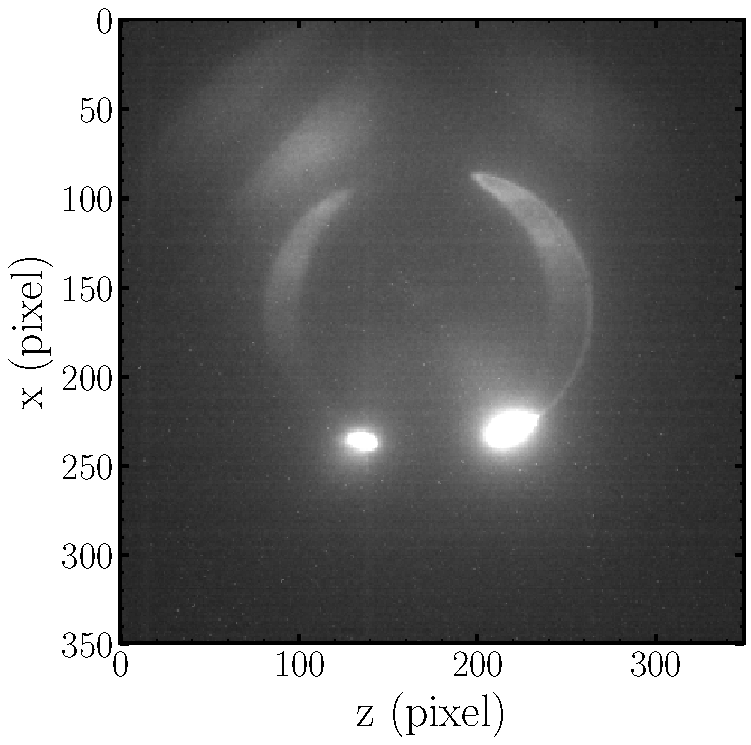
\includegraphics[width=\textwidth]{06_Backup/fig/fig000_FPM_b.pdf}
    \end{column}
  \end{columns}
\end{frame}

\begin{frame}[t]
  \frametitle{Details on extrapolation}
  \begin{block}{Condition}
    \begin{columns}[T]
      \begin{column}{0.45\textwidth}
        ESS nominal:
        \begin{itemize}
          \item $90\,\mathrm{MeV}$ to $2\,\mathrm{GeV}$
          \item $62.5\,\mathrm{mA}$ - $2.86\,\mathrm{ms}$
          \item $10^{-9}\,\mathrm{mbar}$
        \end{itemize}
      \end{column}
      \begin{column}{0.45\textwidth}
        IPHI:
        \begin{itemize}
          \item $3\,\mathrm{MeV}$
          \item $0.7\,\mathrm{mA}$ - $0.05\,\mathrm{ms}$
          \item $4 \cdot 10^{-8}\,\mathrm{mbar}$
        \end{itemize}
      \end{column}
    \end{columns}
  \end{block}
  \begin{tabularx}{\linewidth}{XXXXXXX}
    \toprule    ESS energy (MeV) & Bethe Bloch   & Pressure     & Gas composition & Intensity & Pulse length & Total Signal at IPHI \\
    \midrule
    \(97.2\)                     & $\times 15.5$ & $\times 40 $ & $\times 2.2$    & $\div89$  & $\div57$     & $\times 0.27$        \\
    \(231.4\)                    & $\times 16.4$ & $\times 40$  & $\times 2.2$    & $\div89$  & $\div57$     & $\times 0.28$        \\
    \(278.9\)                    & $\times 29.9$ & $\times 40$  & $\times 2.2$    & $\div89$  & $\div57$     & $\times 0.52$        \\
    \(315.8\)                    & $\times 33.4$ & $\times 40$  & $\times 2.2$    & $\div89$  & $\div57$     & $\times 0.58$        \\
    \(628.3\)                    & $\times 35.8$ & $\times 40$  & $\times 2.2$    & $\div89$  & $\div57$     & $\times 0.62$        \\
    \(2000\)                     & $\times 61$   & $\times 40$  & $\times 2.2$    & $\div89$  & $\div57$     & $\times 1.06$        \\
    \bottomrule
  \end{tabularx}
\end{frame}

\begin{frame}[t]
  \frametitle{Vacuum}
  \begin{block}{Vacuum composition}
    For ions, signal proportion $\neq$ gas proportion. For instance at ESS the $79\,\%$ of $H^{+}_{2}$ in gas represents only one third of the signal.

    Knowing the gas composition during the test is mandatory $\rightarrow$ done with a RGA.
  \end{block}
  \begin{columns}[T]
    \begin{column}{0.45\textwidth}
      Worst case, after an opening:
      \centering
      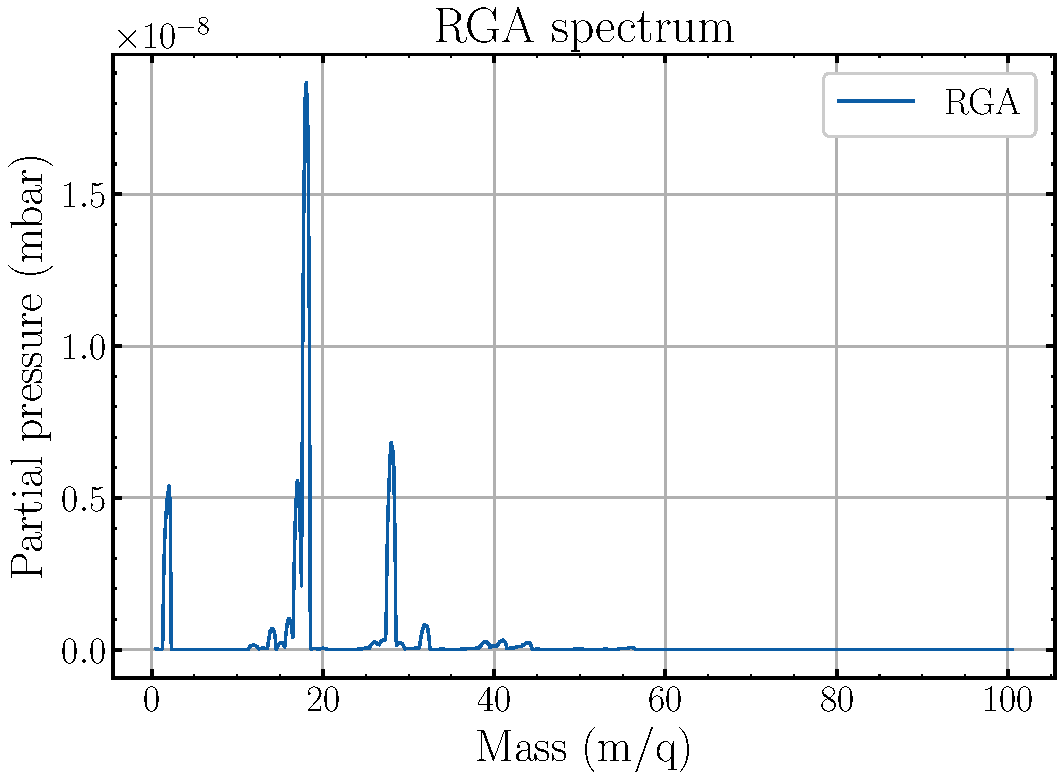
\includegraphics[width=1\textwidth]{06_Backup/fig/fig000_rga_b}
    \end{column}
    \begin{column}{0.45\textwidth}
      Best case, after baking:
      \centering
      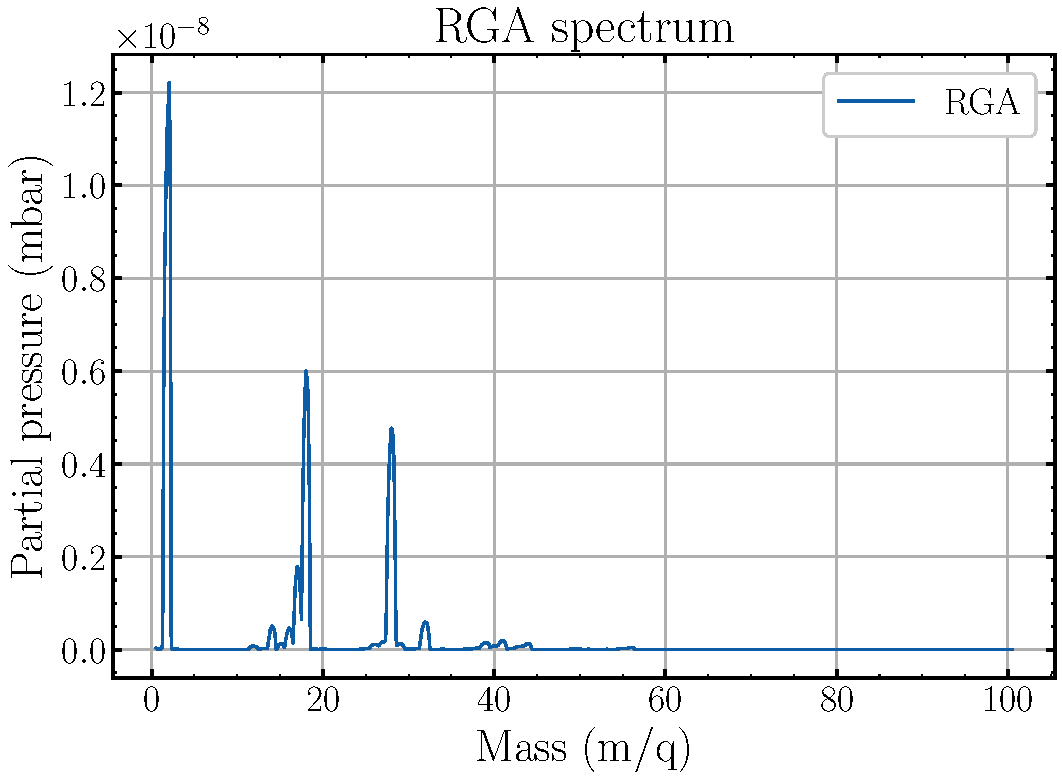
\includegraphics[width=1\textwidth]{06_Backup/fig/fig000_rga_a}
    \end{column}
  \end{columns}

  \begin{alertblock}{Limitation}
    Again vacuum is tricky business, neither gauges or RGA were calibrated.
  \end{alertblock}
\end{frame}

\begin{frame}[t]
  \frametitle{Control system}
  \begin{block}{Experimental Physics and Industrial Control System}
    EPICS is the Control System toolkit used at both ESS and IPHI. The test bench has been integrated to EPICS as much as possible.
  \end{block}

  \begin{columns}[T]
    \begin{column}{0.45\textwidth}
      \begin{block}{Camera}
        PointGrey and AlliedVision
        \begin{itemize}
          \item GigE PoE interface
          \item AreaDetector
          \item ESS fitting plugin
          \item HDF5 file saving
        \end{itemize}
      \end{block}
    \end{column}

    \begin{column}{0.45\textwidth}
      \begin{block}{Power supllies and vacuum}
        Devices from iseg-HV, Inficon, Agilent:
        \begin{itemize}
          \item SCPI TCP
          \item StreamDevice
          \item CSS OPI
        \end{itemize}
      \end{block}
    \end{column}
  \end{columns}

  \begin{alertblock}{CARAMEL}
    Only the CARAMEL board and the FASTER system were not integrated in EPICS.
  \end{alertblock}
\end{frame}

\begin{frame}[t]
  \frametitle{Control system}
  \begin{block}{Introduction}
    Slow control variables for the IPM testbench only $\approx 1000$.

    Useful variables like HV, readout, vacuum, accelerator parameters $\approx 170$
  \end{block}
  \centering
  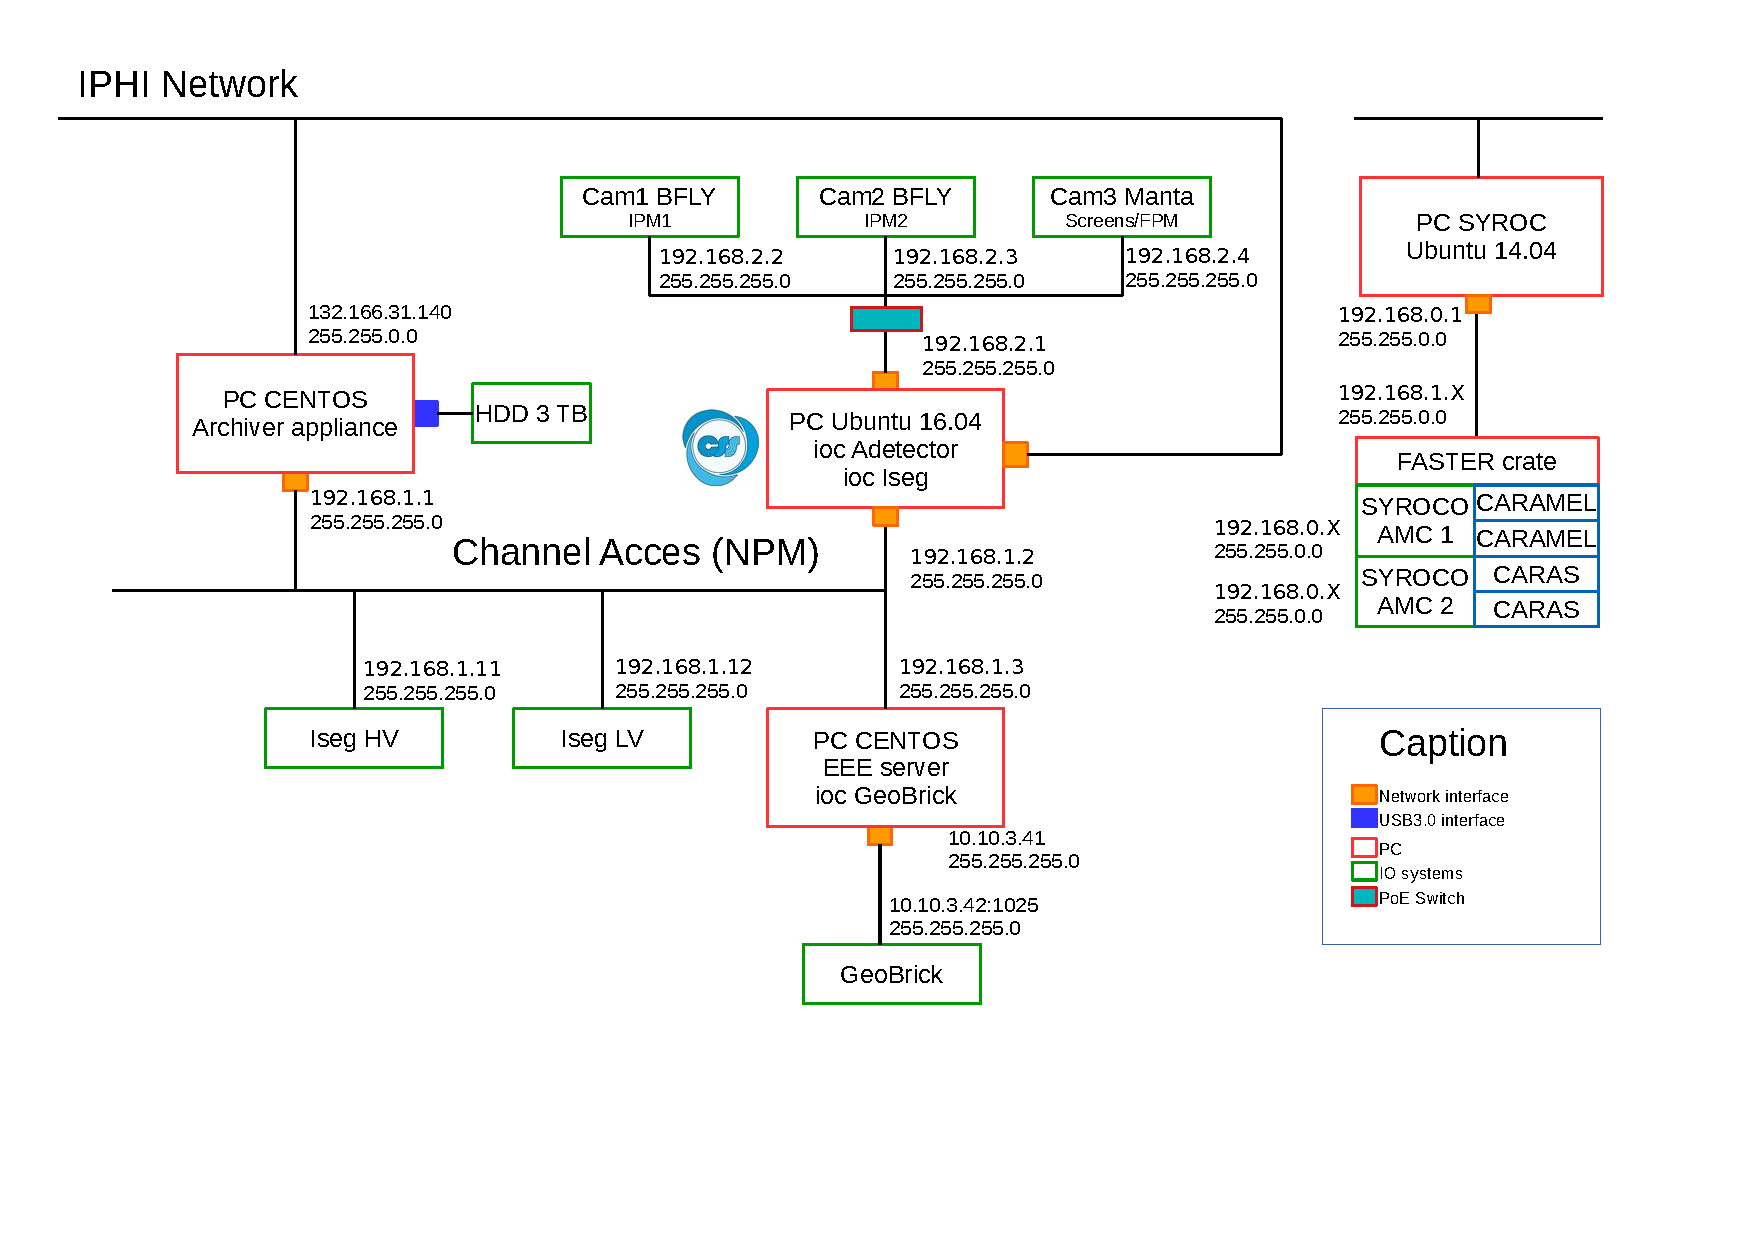
\includegraphics[width=0.9\textwidth]{06_Backup/fig/fig000_EPICS_IPHI.pdf}

\end{frame}